\documentclass[../Main.tex]{subfiles}



\begin{document}

\begin{center}
    \begin{tabular}{| m{1.3 em} | m{0.7\textwidth} | m{0.1\textwidth} |}
    \hline
    1. & Téma bevezetése, ráhangoló kérdések & 5 perc \\
    \hline
    2. & Tanulási fázisok & 5 perc \\
    \hline
    3. & Mind map (gondolattérkép) & 15 perc \\
    \hline
    4. & Cornell módszer & 15 perc \\
    \hline
    - & \textbf{A feladat teljes időtartama} & 40 perc \\
    \hline
    \end{tabular}
\end{center}

\subsection{Bevezetés}

Ebben a részben arról lesz szó, hogy mi a hatékony tanulás, milyen fázisokból áll egy tanulási folyamat,
melyik fázis miért fontos és elengedhetetlen a folyamat során.

\textit{\textbf{Tipp:} Érdemes először a kérdéseket feltenni a gólyáknak, majd hagyni,
hogy agyaljanak rajta és utána közösen megbeszélni (célszerű rávezetni őket a válaszra, akkor jobban elmélyül az új ismeret).} \par

\subsubsection{Miért akar az ember hatékonyan tanulni? \newline Miért fontos a hatékony tanulás?}

Biztos te is hallottad már azt a mondást, hogy a halálod napjáig tanulsz.
Na már most, ha az egész életünk arról szól, hogy tanulunk, akkor lehet nem ártana,
ha ezt jól és hatékonyan tudnánk csinálni.

\textit{\textbf{Rávezető kérdés:} Meddig tanul az ember? Van e vége a tanulásnak az ember életében?}


Fontos, mert ha jól csináljuk, akkor időt tudunk spórolni vele, tovább emlékszünk rá, többek leszünk általa
Rávezető kérdés: Mi lesz az eredménye annak, ha hatékonyan tanulunk? Mit kapunk a hatékony tanulás által?

    
\subsubsection{Mit is jelent az, hogy hatékony tanulás?}

Azt jelenti, hogy valamit képesek vagyunk olyan szinten elsajátítani, hogy egyrészt hosszú távon megmarad,
tehát nem felületes a tudásunk, másrészt tudunk rá építeni, tehát értjük is,
amit megtanultunk és harmadrészt pedig képesek vagyunk felismerni és felhasználni akár a mindennapi életünkben,
akár a munkánk, hivatásunk során.

\textit{\textbf{Rávezető kérdés:} Meddig lenne jó emlékeznünk a megszerzett tudásra? Miért szükséges számunkra az új tudás, mit akarunk vele kezdeni?}

\subsubsection{Hogyan is kell ezt jól csinálni?}
\textit{\textbf{Tipp:} itt elég egy minimális választ megvárni, a kitalálhatóbbakat pl.
 (elegendő idő, elszántság, türelem, kitartás, életünk szerves részévé tevés)
 és utána a többit érdemes hozzáfűzni, mert azok az új ismeretek}

 
Ahhoz, hogy ezt az úgynevezett hatékony tanulást el tudjuk sajátítani, az szükséges hozzá, hogy elszántak,
türelmesek és kitartóak legyünk, biztosítsunk elegendő időt rá, ismerjük a tanulás 5 fázisát,
amire felbomlik, ismerjük mindezekhez a megfelelő tanulási technikákat és ezeket mind az 
életünk szerves részévé tegyük.
 
\textit{\textit{Rávezető kérdés}: Mi szükséges minden jó dologhoz?
 Mit kell tenni ha valami nem sikerül?
 Miből tevődhet össze a tanulás folyamata?}

 \subsubsection{De mi is ez az 5 fázis? \newline Melyik mit takar? \newline Miért fontos része a tanulási folyamatnak?}



\begin{enumerate}
    \item {Tervezés}
    \begin{enumerate}
        \item {Mit csinálsz ekkor?}
        \begin{enumerate}
            \item legelső lépés legyen mindig az, hogy megtervezed a tanulási folyamatodat
            \begin{enumerate}
                \item Melyik tantárgy?
                \item Melyik anyagrész?
                \item Melyik nap?
				\item Mennyi időd van rá?
				\item Meddig akarsz eljutni vele aznap?
            \end{enumerate}
        \end{enumerate}
        \item Miért fontos ez?
        \begin{enumerate}
            \item mert így be tudod iktatni a hétről, hétre tanulást, ami a sikeres és hatékony tanulás egyik kulcsa
            \item mert így tisztábban fogod látni, hogy mikor meddig kell eljutnod ahhoz, hogy megtudd tanulni az anyagot
                 időre, ami segít a koncentrációdon is, mert akkor tényleg csak arra tudsz fókuszálni, ami aznapra van
        \end{enumerate}
    \end{enumerate}

    \item Előkészület
    \begin{enumerate}  
        \item Mit csinálsz ekkor?
        \begin{enumerate}
            \item elhelyezed magadat az adott témában
            \begin{enumerate}
                \item áttekinted a teljes nagy anyagrészt
                \item elolvasod az aznapra kijelölt anyagrészt
            \end{enumerate}
        \end{enumerate}
        \item Miért fontos ez?
        \begin{enumerate}
            \item mert ezzel kicsit belerázódsz az anyagba, ráhangolódsz
			\item mert ezzel már egy kicsit megismerkedsz a megtanulandó résszel
		\end{enumerate}
    \end{enumerate}
    \item Megértés
    \begin{enumerate}
        \item Mit csinálsz ekkor?
        \begin{enumerate}
            \item megpróbálod megérteni az anyagrészt
            \begin{enumerate}
                \item han em sikerül magadtól, akkor KÉRJ segítséget!!!
                \begin{itemize}
                    \item tanártól
					\item szaktárstól
					\item Internet
					\item könyvtár
					\item EIK-esek (eotvos.informatikai.kor@gmail.com)
                \end{itemize}
            \end{enumerate}
            \item megpróbálod összekapcsolni korábbi ismeretekkel, hogy tudd hova kötni
            \begin{enumerate}
                \item korábbiak elolvasása
			    \item kapcsolatok megkeresése
            \end{enumerate}
        \end{enumerate}
        \item Miért fontos ez?
        \begin{enumerate}
            \item mert ha értjük és már tudjuk hova kötni az új tudást, akkor könnyebben tudjuk megtanulni
			\item mert így könnyebben tudjuk felhasználni ott, ahol szükséges
        \end{enumerate}
    \end{enumerate}

    \item Megtanulás
    \begin{enumerate}
        \item Mit csinálsz ekkor?
        \begin{itemize}
            \item elsajátítod annyira az anyagot, hogy segédanyag nélkül is TUDOD
		    \item TUDOD = fel tudod pontosan idézni, érted, tudod alkalmazni, tudsz hozzá kapcsolni új dolgokat
		    \item ha ezek közül akár csak egy nem teljesül, akkor még nem tanultad meg!
        \end{itemize}
        \item Miért fontos ez?
        \begin{itemize}
            \item mert így rögzül az agyadban hosszútávra
        \end{itemize}
    \end{enumerate}

    \item Visszaidézés
    \begin{enumerate}
        \item Mit csinálsz ekkor?
        \begin{enumerate}
            \item megpróbálod visszamondani a tanultakat
        \end{enumerate}
        \item Miért fontos ez?
        \begin{itemize}
            \item mert ezzel megtanuljuk előhívni a megszerzett tudást
            \begin{itemize}
                \item egy dolog bejuttatni az agyba az információt és megint másik dolog azt az információt előhívni
                \begin{itemize}
                    \item más idegi pályákon történik a bejuttatás és az előhívás, ezért fontos mindkettőt gyakorolni
                    \begin{itemize}
                        \item amíg még friss a bejuttatott információ addig könnyebben tudunk rá emlékezni így hamar ki
                         tudjuk építeni azt az idegi pályát, amin majd a későbbiekben is elő tudjuk hívni az új ismeretet
                        \item gyakorlással mélyítjük el az idegi pályákat
                    \end{itemize}
                    \item minél mélyebb, többször bejáratot az idegi pálya annál tartósabban, hosszabb ideig megmarad az információ
                \end{itemize}
            \end{itemize}
        \end{itemize}
    \end{enumerate}
\end{enumerate}


\subsection{Mind map, avagy a gondolattérkép}

Ebben a részben arról lesz szó, hogy miért hatékony a mind map, mire szolgál és hogyan épül fel.

\subsubsection{Mi az a Mind map?}

\textit{\textbf{Tipp:} érdemes először a kérdéseket feltenni a gólyáknak, majd hagyni,
 hogy agyaljanak rajta és utána közösen megbeszélni 
(célszerű rávezetni őket a válaszra,akkor jobban elmélyül az új ismeret).} \newline
 \textit{\textbf{Rávezető kérdés:} Mi az a mind map?} \newline
\textit{\textbf{Tipp:} Ha valaki már ismeri kérjük meg, hogy foglalja össze pár mondatban}

Magyarul a Mind Map Gondolattérképet jelent. Ez egy olyan tanulási eszköz, amelynek az egyszerűségében és
az egységes egészben való ábrázolásban(holisztikus gondolkodás) rejlik a szépsége. Papíron egy gyönyörű
diagram szemlélteti a témához fűződő információkat (összefüggéseket).
A mind map az elemi tanulási technikák közé tartozik, hiszen a kulcsfogalmakat emeljük ki
és foglaljuk össze ábrák készítésével és a fogalmak közötti kapcsolatok felfedezésével.
Nagyon hasznosnak minősül, mivel szinte az összes tanulási típust (például: auditív, vizuális, taktilis) lefedi.
Ez a tanulási módszer aktiválja az “egész” agyunkat, ahogyan a logikáért felelős bal oldali agyféltekét,
úgy a kreativitásért felelős jobb oldali agyféltekét is. Következtetés képen egy nagyon hatékonyés szórakoztató módszer.

\subsubsection{Mikor érdemes ezt a technikát használni? \newline Hasznos vele előadást jegyzetelni?}

Előadás közbeni jegyzetelésre nem hasznos.
Használjuk azután miután már van egy alap jegyzetünk, hiszen limitált helyünk van és azt jól kell beosztani.
    Hasznos egy dolgozat előtt felvázolni/ feltérképezni a témát. Segít átlátni a ZH anyagát egy nagy egységben.

\subsubsection{Mind map elkészítése}

\textit{\textbf{Feladat:} A gólyák alkossanak csoportokat (2-3 fő).
Kapjanak egy A4-es fehér lapot és legalább 5 színes ceruzát.
Kérjük meg, hogy egyezzenek meg gyorsan egy témán, amit lépésenként együtt dolgoznak ki.
Míg prezentáljuk a lépéseket ők dolgozzanak.}

\textbf{Lépések}

\begin{enumerate}
    \item Helyezzük el a papírt magunk előtt (horizontálisan).
    Rajzoljunk egy képet (esetleg írjunk fel egy címet) a közepére ami az egész témát jelöli.
    \textbf{FONTOS:} A rajzhoz legalább három színt használjanak.

    \item Válasszunk egy színt és rajzoljuk meg a fő témádból kiinduló első törzset.
    Ez azért jó mert a törzs vastagsága szimbolizálja a kulcsszó asszociációs rangját (hierarchy).

    \item Címezzük fel a törzset nagybetűkkel és ugyanazzal a színnel, amivel megrajzoltuk.
    (A címzés helyett használhatsz kis ábrákat is.)

    \item Ismételgessük a 2., 3., 4. lépéseket, amíg végig nem érünk a témán. Figyeljünk arra, hogy egyenletesen osszuk el a rendelkezésedre álló teret törzsenként.
   
\end{enumerate}
\textit{\textbf{Tipp:} Elég, ha 2-3 törzset berajzolnak.} \newline
\textit{\textbf{Extra:} Ha két törzs között találunk valamilyen kapcsolatot akkor ne
féljünk egy nyíllal azt megjelölni ,és leírni az összefüggés kulcsszavát a nyíl felé.} \newline
\textit{\textbf{Tipp:} Ha van egy bátor, vállalkozó szellemü hallgató, akkor kérjük meg,
hogy összefüggő mondatokban prezentálja a megrajzolt gondolattérképét. Ha nincs jelentkező,
akkor bátorítsuk őket és kérjünk meg valakit.}

\subsubsection{\textit{Nem kötelező de ajánlott:} Mind map előnyei és hátrányai}

\textbf{Előny}

Segít a rendszerezésben.
Segítségével felrajzolhatjuk a tananyagban talált kapcsolatokat.
Látványos.(színes, képek kombinációja szavakkal/kifejezésekkel)
Megjelenik benne az asszociációs logika.
Több szemszögből is megtekinthető, multidimenzionuális.
Elemei általában “buborékok”, körök (általában a fogalmakat jelölik) és őket összekötő vonalak 
(a fogalmak közötti kapcsolatok jelölésére).
Használhatunk egyéb jelöléseket, színeket - bármit, ami segít.

\textbf{Hátrrány}

Érdemes rá figyelni, hogy ne legyen nagyon bonyolult rajzunk, mert így a módszer veszíthet a hatékonyságából.
Figyelni kell a jelölések rendszerezésére, mert átláthatatlanná válik.
Nem szabad hosszú szövegeket felírni.
Óra közben ne ezt a módszert használjuk jegyzetelésre, mert limitált helyünk van
Figyelni kell a rendszerezésre és a témák megfelelő elosztására

\textit{\textbf{Téma lezárásához:} Elmondhatjuk, hogy matektanulásban a definíciók, tételek, bizonyítások megértésében segít, illetve a feladat megoldási menetének megértése/ feltérképezésében is.
+ További információért felírhatjuk Tony Buzan nevét a táblára, ha rákeresnek találnak irodalmat és szoftvert is a témához!}

\subsection{A Cornell módszer}

\subsubsection{Bevezetés}


A Cornell módszert az amerikai Cornell University egyetemen tanító professzor, Dr.
Walter Pauk fejlesztette ki és tökéletesítette. Célja az volt, hogy egy átfogó rendszert
alkosson jegyzetelésre, tanulásra és memorizálásra. Használatával jól strukturált,
átlátható, könnyen tanulható és jól visszakereshető jegyzeteket készíthetünk és eközben
agyunk olyan területei dolgoznak, amik passzív módszerek használata során nem.


\subsubsection{Hogyan készítsünk Cornell jegyzeteket?}

A Cornell módszer alapja rendkívül
egyszerű – hagyjunk széles margókat a
papíron, pontosabban 3 széles margót: egyet a
lap tetején, egyet a lap bal oldalán, egyet a lap
alján. A maradék rész (legnagyobb a papíron)
az előadáson vagy gyakorlaton leírt jegyzetek
helye. Ajánlott valamilyen behúzási,
címkézési (számozás, jegyzetpontok) szabályt
itt is követni, hogy a szövegtörzs is olyan
átlátható legyen mint a teljes dokumentum.
Tanácsos azonban jegyzetelésnél egy oszlopra
korlátozni magunk, a későbbi kiegészítés
miatt.

\begin{wrapfigure}{r}{0.5\textwidth}
    \centering
    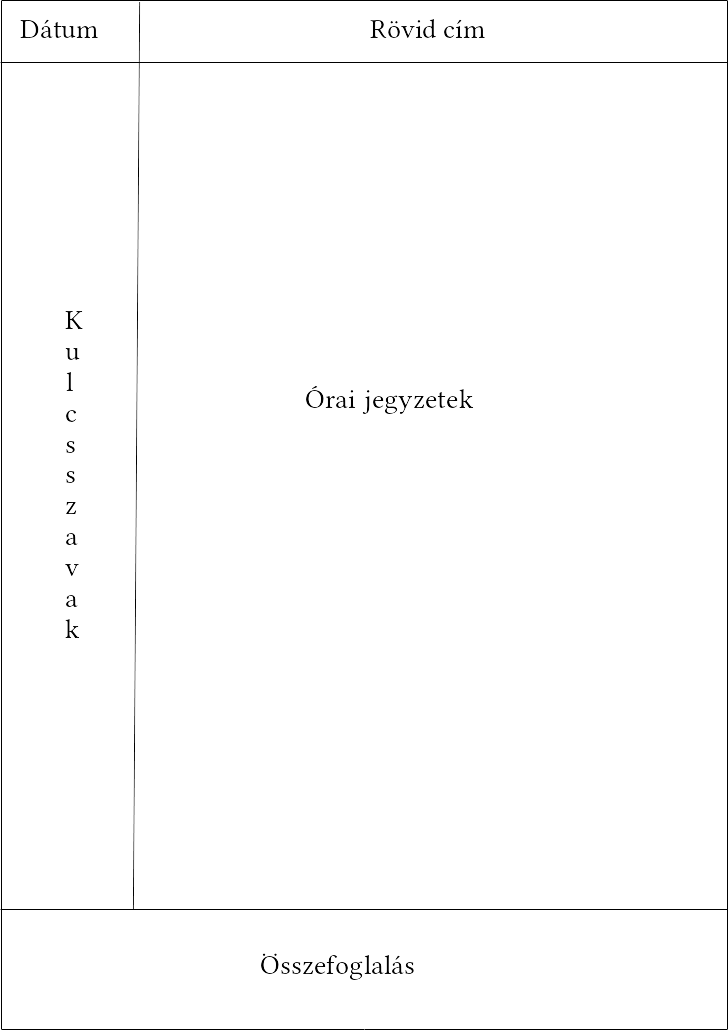
\includegraphics[width=0.48\textwidth]{Cornell}
    \caption{Cornell jegyzetlap felosztása}
    \end{wrapfigure}
    
A szövegtörzstől balra lesznek majd a
kiemelt kulcsszavak, fontosabb megjegyzések,
alcímek, esetleg kérdések. A lehetőségek
tárháza nagy, nincs pontos szabály arra, hogy
pontosan mi legyen ebben a részben. Dr. Walter
Pauk könyvében a kérdéseket-, míg más források 
inkább a kulcsszavakat ajánlják, célszerű azonban
pár szóra szorítkozni minden esetben.



A kulcsszavak a vele egy sorban álló szövegtörzs kiemelése, egy-két szóban való
megfogalmazása, ezért is fontos, hogy ne két oszlopban jegyzeteljünk, mert így nem
egyértelmű, melyik oszlophoz tartozzon a szó.
 A Cornell jegyzetek alján egy 3-4 soros összesítés található teljes mondatokban. Ebben
a számunkra új és hasznos információkat összegezhetjük nyelvi közlés szintjén. Ne
akarjuk az egész jegyzet tartalmát itt felsorolni, törekedjünk a rövidségre.
A lap tetejére kerül a jegyzet címe és az előadás vagy gyakorlat dátuma, amin a
szövegtörzset elkészítettük. A jegyzetek átrendezését, konkrét adatok keresését nagyban
meggyorsítja, ha a lap tetejére nézve tudjuk milyen témakörbe esik a jegyzet tartalma.
Ebbe a részbe tartozhat még a foglalkozás megnevezése (előadás vagy gyakorlat) is.


\subsubsection{Előnyök}


Ahhoz, hogy jó Cornell jegyzeteket készítsünk, nem elég csak az előadáson jegyzetelni.
A jegyzetek kiegészítése lehetőséget ad arra, hogy tisztában legyünk a pontos anyaggal,
értsük a felépítést, összefüggéseket. Legnagyobb előnye, hogy nagy odafigyelést és
közvetlen bevonódást igényel. Amikor kiemeljük a kulcsszavakat, pontosan meg kell
néznünk, mi áll az adott sorban és hogyan lehetne egy-két szóban megfogalmazni, tehát
értenünk kell miről szól a szöveg, nem elég rápillantani. Itt arra is alkalmunk akad, hogy a
le nem írt gondolatokat az előadásról valahogyan dokumentáljuk vagy kérdéseket tegyünk
fel, ha valamit nem értünk. Ugyanakkor kritikus gondolkodást is igényel részünkről. Ha
hiányos valahol a jegyzet, vagy esetleg elírás van, az azonnal feltűnik és idejében
javítható. Összességében, mély megértésre ösztönöz minket a jegyzet ilyesfajta
összefoglalása. Ha már tudjuk milyen kulcsszavakat tartalmaz a jegyzet, meg tudjuk
fogalmazni a teljes oldal tartalmát saját szavainkkal, lefordítva ezzel saját nyelvünkre.
A jegyzetek erejében a kiegészítés rejlik, ezért ne féljünk rászánni a megfelelő időt. Ezt
ajánlott az előadás utáni első szabad alkalommal megtenni, mert ilyenkor még tisztábban
emlékszünk az előadás részleteire. A kiegészítésnek van egy elsőre nem látható haszna is:
megörökíti azokat a lépéseket aminek segítségével eljutottunk a megértésig. Hányunkkal
megesett már, hogy megértettünk egy matematikai összefüggést, de két héttel később
ismét percekig kellett elemeznünk a képletek? A Cornell módszer ebben is segít. Mivel mi
írtuk és egészítettük ki a jegyzeteket, akaratlanul is a mi gondolkodásunkat fogja tükrözni,
ezért is használhatók remekül később, amikor nagy dolgozatra készülünk.



Ne feledkezzünk meg arról a tényről sem, hogy a jegyzetkészítés és kiegészítés alatt
rengeteget írtunk, egy információmorzsát többször is feldolgoztunk (először kulcsszavak
kiemelésében, másodszor az összefoglalás megírásában). Kutatások kimutatták, hogy azok
a diákok akik tollal jegyzeteltek papírra, hetekkel az előadás után jobban szerepeltek a
kutatócsoport tesztjeink mint azok, akik laptopot vagy más elektronikus eszközöket
használtak. Ahhoz hogy a beszélt szövegből írott jegyzet legyen, már szükséges egy fajta
fordítás a mi részünkről. Sok esetben nem tudunk leírni teljes bekezdéseket, mert az
előadás tempója nem teszi ezt lehetővé, emiatt tudatosan csak a lényegre kell
koncentrálnunk.

Agyunk számára az írás soha nem monoton tevékenység. A betűk megformálását, a sor
tartását, a szavak elválasztását és ez extra formázásokat mind gyors egymásutánban
végezzük, nem hagyhatunk semmit az utómunkára. Ha valamit elrontottunk, azt már
nehéz kitörölni és átfogalmazni, nem úgy mint egy számítógép szöveges szerkesztőjében.
Ez tudatos előre gondolkodást igényel a jegyzet készítőjétől. Ha strukturáltan le tudtuk
írni kézzel, akkor a fejünkben is rendezettebben tároltuk el az előadás anyagát.


\subsubsection{Hátrányok}


    A módszer hatékonyságát a belefektetett idő erősen befolyásolja. Attól függően, hogy
hetente ki mennyit jegyzetel, akár 20-30 oldal összegyűlhet egy hét folyamán. Ennyi
jegyzetet sok idő kiegészíteni és felcímkézni, nem is beszélve arról, hogy ezt nem
mindenhol tehetjük meg. A folyamat nagy koncentrációt igényel és ki tudja fárasztani az
elmét pár óra alatt. A folyamat során gyakran megtörténik, hogy egy információt több
helyen is leírunk: a jegyzetben, a kulcsszavak között és az összefoglalásban. Ez a tárolási
mód erősen redundáns, ezért a jegyzet nehezen használható kidolgozott rövid
összefoglalóként.

Bár a módszer alapja meglehetősen egyszerű, nehéz hozzászokni azoknak akik nem
hasonló rendszereket használtak korábban. Először feleslegesnek és szokatlannak tűnhet,
hogy miért írjuk le ugyanazt az információt a kulcsszavak közé, ami a jegyzetben már
szerepel, nem is beszélve az összefoglalásról. Bár a módszer első használatra
körülményesnek tűnhet, hosszú távon nagy előnnyel jár, ha valaki rendszeresen használja
és kiegészíti.


\subsubsection{Hol használható a matematika tanulásban?}


A Cornell módszer a tantárgyak mindegyikében nagy segítséget nyújt, különösképpen a
gyakorlati alkalmazásokat igénylőknél. A matematika nem csak a logikánkat teszi próbára,
de akadályt jelenthet az absztrakt, bonyolult képletek alkalmazása egyszerű feladatokra, és
a tételbizonyítások lépéseit is nehéz megjegyezni. A felsorolt akadályok mindegyikében
segítségünkre lehet a Cornell módszer.

\textbf{Logika megértése}



    A matematikai levezetések és tételalkalmazások alapja, hogy a különböző állítások
erősségével (szükséges, elégséges, szükséges és elégséges) és az azok közötti
összefüggésekkel tisztában legyünk. A kiegészítés összefoglalójában leírhatjuk ezeket,
vagy a kulcsszavak között rövid tőszavak, szimbólumok segítségével jelölhetjük a tételek
közötti összefüggéseket. Ha valamit nem értünk, vagy nem értelmes az adott
kontextusban, a kiegészítés alatt kiderülhet. A rossz irányú implikáció, kihagyott vagy
rossz logikai kvantor, rossz indexelés mind olyan hiba, amit csak nagy figyelemmel lehet
észrevenni és javítani. Szerencsére a kulcsszavak kiemelésénél tüzetesen át kell néznünk a
jegyzetpontokat. Szánjunk időt ezekre a javításokra!

\textbf{Tételek alkalmazása, bizonyítása}


A gyakorlatokon alkalmazott tételek absztrakt jellegéből adódóan nehezen
megfogalmazhatók, sokszor nem egyértelmű milyen helyzetben használhatók. A tételek
feltételeit és állításait mind kiírhatjuk a kulcsszavak közé (ha folytonos függvény...,
deriválható függvény..., ...ekkor van inverz mátrix stb.), ezzel a tételt saját szavainkkal
leegyszerűsítettük „ha ez és ez adott, akkor ezt és ezt mondhatjuk” alakra, ami már sokkal
közelebb áll az alkalmazáshoz. Egyes állítások, levezetések több lépésesek lehetnek. Az
ilyen hosszú gyakorlati levezetések fontos lépéseit kiemelhetjük a kulcsszavak közé, így
egy átfogó képet kaphatunk az általános lépésekről, mindezt a saját szavainkkal.
Tételek bizonyításának mindig van 1-2 kulcslépése, ami nem magától értetődő, ezeket
mindenképp memorizálni kell. Ebben is segítségünkre van a Cornell módszer, mert az
esetleges 3-szoross rögzítéssel (jegyzet, kulcsszó, összefoglalás) sokszor már további
memorizálás nélkül megmarad ez a kulcsinformáció.


\end{document}